\documentclass[11pt,a4paper]{uebung}

\usepackage[british]{babel}
\usepackage{epsfig}
\usepackage{rotate}
\usepackage{amsmath,amsthm,amssymb}
\usepackage{color}
\makeatletter\let\@amsfonts=P\makeatother
\usepackage{graphicx}
\usepackage{typearea}
\usepackage{multicol}
\usepackage{amsfonts}
\usepackage[nounderscore]{syntax}
\usepackage{paralist}
\usepackage{enumitem}
\newcommand{\comment}[1]{\marginpar{\small{\bf Comment:} #1}}

\usepackage{tikz}
\usetikzlibrary{shapes,arrows,backgrounds,%
matrix,patterns,arrows,decorations.pathmorphing,decorations.pathreplacing,%
positioning,fit,calc,decorations.text,shadows%
}

\newcommand{\solution}[1]{\par {\bf Solution:}\\#1}
\def\impl{\rightarrow}

%%%
% put your Matrikelnummer here instead of the XXXXXXXX
%%%
\newcommand\matrikelnummer[0]{XXXXXXXX}
%%%
% put your Matrikelnummer here instead of the XXXXXXXX
%%%

\newcommand{\nop}[1]{}

\def\cT{\mathcal{T}}


\begin{document}
\newcommand{\Vorlesung}{Formal Methods in Computer Science}
\newcommand{\Semester}{SS 2013}
\newcommand{\Prof}{Uwe Egly}
\newcommand{\AssisA}{Antonius Weinzierl}
\newcommand{\AssisB}{}

%%%%%%%%%%%%%%%%%%%%%%%%%%%%%%%%%%%%%%%%%%%%%%%%%%%%%%%%%%%%%%%%%%%%%%%%%%%%%%

\Uebungsblatt{Block 2}{Matrikelnummer: \matrikelnummer}

%%%%%%%%%%%%%%%%%%%%%%%%%%%%%%%%%%%%%%%%%%%%%%%%%%%%%%%%%%%%%%%%%%%%%%%%%%%%%%


If you would like to receive feedback \emph{in the exercise sessions}, you
should submit your solutions to TUWEL no later than \emph{May 10th 2013}. If
you upload you exercises up to \emph{May 20th 2013}, you will get feedback in
electronic form.
\\ \\
This exercise sheet is divided in two parts: first algorithms and techniques,
second proofs and properties. Since the questions of Block 2 of the final exam
are going to have a strong emphasis on understanding and proofs, it is highly
recommended to train \emph{at least} on the exercises of the second part.

\section{Algorithms and Techniques}


\Aufgabe[First-Order Theories]

To get an intuition, what a formula means, it often helps to visualize an
example instantiation of the occuring relations. That is, one visualizes a
model (or interpretation) of the formula by drawing the respective relations.
Binary relations can be visualized very easily as directed
graphs: let $R \subseteq U \times U$ be a relation on the $U$, then
the corresponding directed graph $G$ is $G=(U,R)$. So, whenever two elements
$u_1$ and $u_2$ of the universe of an interpretation are related by $R$, then
the corresponding graph contains an edge between $u_1$ and $u_2$.

For example, the graph in Figure \ref{fig:graph_transitive} shows a
transitive relation, i.e., the relation $R$ satisfies the following formula
$\forall x \forall y \forall z : x R y \land y R z \rightarrow x R z$. So the
graph is a visualization of one model of the formula.
\begin{figure}[ht]
  \centering
  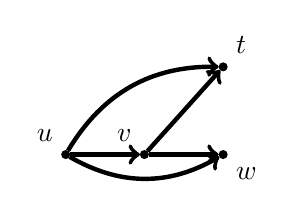
\begin{tikzpicture}[v/.style={circle,draw,fill,inner sep=1}]
    \node[v,label=above left:$u$] (u){};
    \node[v,right of=u,label=above left:$v$] (v){};
    \node[v,right of=v,label=below right:$w$] (w){};
    \node[v,above=of w,label=above right:$t$] (t){};
    \draw[line width=1.6pt,->] (u) -- (v);
    \draw[line width=1.6pt,->] (v) -- (w);
    \draw[line width=1.6pt,->] (u) edge [bend right] (w);
    \draw[line width=1.6pt,->] (v) -- (t);
    \draw[line width=1.6pt,->] (u) edge[bend left] (t);
  \end{tikzpicture}
  \caption{A graph visualizing the transitive relation $R= \{ (u,v), (v,w),
    (u,w), (v,t), (u,t) \}$. The corresponding interpretation (with universe
    $U=\{u,v,w,t\}$) is a model of the formula $\forall x \forall y \forall z
    : x R y \land y R z \rightarrow x R z$.}
  \label{fig:graph_transitive}
\end{figure}

\begin{enumerate}
\item Let $T_1$ be a theory consisting of the following fomulae:
  \begin{align*}
    \forall x: x R x\\
    \forall x \forall y: x R y \rightarrow y R x
  \end{align*}
  \begin{enumerate}
  \item Pick a domain of size at least $5$, pick any model of $T_1$ based on
    your chosen domain, and visualize $R$.
  \item Consider the following graph, and extend it such that it corresponds
    to a model of $T_1$.

  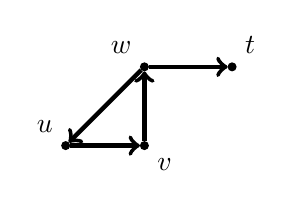
\begin{tikzpicture}[v/.style={circle,draw,fill,inner sep=1}]
    \node[v,label=above left:$u$] (u){};
    \node[v,right of=u,label=below right:$v$] (v){};
    \node[v,above of=v,label=above left:$w$] (w){};
    \node[v,right=of w,label=above right:$t$] (t){};
    \draw[line width=1.6pt,->] (u) -- (v);
    \draw[line width=1.6pt,->] (v) -- (w);
    \draw[line width=1.6pt,->] (w) -- (u);
    \draw[line width=1.6pt,->] (w) -- (t);
  \end{tikzpicture}
  \item Visualize a relation, which violates $T_1$.
  \end{enumerate}

\solution{

}

\item Visualize the theory $T_2$, which consists of the formula:
  \begin{align*}
    \forall x \exists y: x R y
  \end{align*}
  \begin{enumerate}
  \item Pick a domain of size at least $5$ and visualize a chosen model of
    $T_2$.
  \item Consider the following graph, and extend it such that it corresponds
    to a model of $T_2$.

  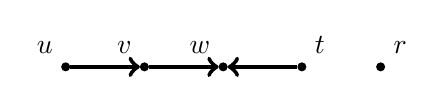
\begin{tikzpicture}[v/.style={circle,draw,fill,inner sep=1}]
    \node[v,label=above left:$u$] (u){};
    \node[v,right of=u,label=above left:$v$] (v){};
    \node[v,right of=v,label=above left:$w$] (w){};
    \node[v,right of=w,label=above right:$t$] (t){};
    \node[v,right of=t,label=above right:$r$] (r){};
    \draw[line width=1.6pt,->] (u) -- (v);
    \draw[line width=1.6pt,->] (v) -- (w);
    \draw[line width=1.6pt,->] (t) -- (w);
  \end{tikzpicture}
  \end{enumerate}

\solution{

}

\end{enumerate}


\Aufgabe[Tseitin Transformation]

\begin{enumerate}
\item For the formula $\psi= \big(a \rightarrow ( b \rightarrow \neg a)\big)$
  use Tseitin to compute a sat-equivalent CNF.

\solution{

}

\item Given the circuit below with AND, NAND, and OR gates, use Tseitin to
  obtain a linear-size CNF.

  \begin{figure}[h!]
    \centering
    \begin{tikzpicture}
      \begin{scope}[scale=0.75]
        \node[rectangle,draw,minimum height=1.4cm,minimum width=1cm]
        (nand) at (2.5,3) {$\wedge$};
        \node[circle,draw,anchor=west] (nandneg) at (nand.east) {};
        \node[rectangle,draw,minimum height=1.4cm,minimum width=1cm]
        (andl) at (2.5,1) {$\wedge$};
        \node[rectangle,draw,minimum height=2cm,minimum width=1cm]
        (or) at (5,2) {$\vee$};
        \node[rectangle,draw,minimum height=2.5cm,minimum width=1cm]
        (andr) at (7,0.75) {$\wedge$};
        \node[circle,draw,anchor=west] (andneg) at (andr.east) {};
        \draw (nandneg.east) -- ($(or.north west)!(nand.east)!(or.south west)$);
        \draw (andl.east) -- ($(or.north west)!(andl.east)!(or.south west)$);
        \draw (or.east) -- ($(andr.north west)!(or.east)!(andr.south west)$);
        \node (inx) at (0.5,3.5) {$x$};
        \node (iny) at (0.5,2.5) {$y$};
        \node (inz) at (0.5,0.5) {$z$};
        \draw (inx.east) -- ($(nand.north west)!(inx.east)!(nand.south west)$);
        \draw (iny.east) -- ($(nand.north west)!(iny.east)!(nand.south west)$);
        \draw (inz.east) -- ($(nand.north west)!(inz.east)!(nand.south west)$);
        \draw (iny.east) -- ++(0.5,0) -- ++(0,-1) coordinate (tmp1) --
        ($(nand.north west)!(tmp1)!(nand.south west)$);
        \draw (andl.east) -- ++(0.5,0) -- ++(0,-1) coordinate (tmp2) --
        ($(andr.north west)!(tmp2)!(andr.south west)$);
        \node (out) at ($(andneg.east)+(1,0)$) {$o$};
        \draw (andneg.east) -- (out.west);
      \end{scope}
    \end{tikzpicture}
  \end{figure}
  
  
\solution{

}

\end{enumerate}

\newpage

\Aufgabe[Implication Graphs]


Let $\mathcal{C}$ be a clause set consisting of the following clauses:

\begin{eqnarray*}
  c_1 \colon &&( \neg A \lor B )\\
  c_2\colon &&( \neg A \lor \neg B \lor C )\\
  c_3\colon &&( A \lor B )\\
  c_4\colon &&( \neg F \lor \neg B \lor \neg G )\\
  c_5\colon &&( G \lor \neg E )\\
  c_6\colon &&( G \lor D )\\
  c_7\colon &&( C \lor E \lor \neg D )\\
  c_8\colon &&( \neg A \lor C )
\end{eqnarray*}

\begin{enumerate}
\item Draw an implication graph for $\mathcal{C}$. Use the decision $C=0@1$,
  and $F=1@2$ until you reach a conflict.


\solution{

}

\item Determine all UIPs in the implication graph, find the first UIP and use
  resolution to learn a conflict clause corresponding to the first UIP.

\solution{

}

\item Add the learned clause, apply conflict-driven backtracking and draw the
  resulting implication graph.

\solution{

}
\end{enumerate}


\Aufgabe[Sparse Method]
Apply the Sparse Method including preprocessing on the formula $\varphi$
below to obtain a propositional formula. Note that $\varphi$ is not yet in NNF
(Negation Normal Form).
\begin{displaymath}
  (x_1 = x_2 \rightarrow x_2=x_3) \land
  \big[ \neg (x_2 = x_4 \lor x_3 \neq x_4
  \lor x_4 \neq x_5)
  \lor (x_6 \neq x_5 \land x_6=x_7 \land x_7=x_3)\big]
\end{displaymath}

\solution{

}


\Aufgabe[Ackermann's Reduction]
Apply Ackermann's reduction on the following EUF-formula $\varphi$ to obtain
an E-formula:
\begin{gather*}
  F(F(x_1)) \neq F(x_1) \land G(x_1,x_2) = F(x_2) \land F(G(x_2,F(x_2))) \neq F(F(x_1))
\end{gather*}

\solution{

}



\newpage
\section{Proofs and Properties}

\Aufgabe[First-Order Theories]
\newcommand{\caT}{{\cal T}}
\newcommand{\semder}{\models}
In the lecture, we discussed reasoning under different theories. Here we are
concerned with LISP-like lists and the theory $\caT_{\mathit{cons}}^E =
\caT_{\mathit{cons}}\cup \caT_E$.  In a verification attempt of some program,
we have to prove the following:
\begin{center}
\begin{minipage}{0.8\textwidth}
{\em For non-atomic lists $\ell_1, \ell_2$, if the ``car'' of both lists are
  equal and the ``cdr'' of both lists are equal, then $\ell_1$ is equal to
  $\ell_2$.  }
\end{minipage}
\end{center}
We formalize the above statement as follows:
$$ \varphi \colon \quad
\big[\, \neg \textit{atom}(\ell_1) \land \neg \textit{atom}(\ell_2) \land 
\textit{car}(\ell_1)  \doteq \textit{car}(\ell_2) \land  
\textit{cdr}(\ell_1) \doteq \textit{cdr}(\ell_2) \, \big] \,\, 
\impl \,\,  \ell_1 \doteq \ell_2  
$$
Prove the statement $\caT_{\mathit{cons}}^E$-valid, i.e., show that
$\caT_{\mathit{cons}}^E \semder \varphi$.

\medskip

Hint: Besides the equality axioms reflexivity, symmetry and transitivity, the
following axioms from $\caT_{\mathit{cons}}^E$ are sufficient for a proof:
\begin{itemize}

\item[(1)] Substitution axioms (functional congruence) for
  $\textit{cons}$: 

  $$\forall x_1\forall x_2 \forall y_1 \forall y_2 \, [
(x_1 \doteq x_2 \land y_1 \doteq y_2) \impl   
\textit{cons}(x_1,y_1) \doteq \textit{cons}(x_2,y_2)]$$
\item[(2)] Construction:
$$\forall x\, [\neg \textit{atom}(x) \impl 
\textit{cons}(\textit{car}(x), \textit{cdr}(x)) \doteq x] $$ 

\end{itemize}

\solution{
}


\Aufgabe[Tseitin Transformation]
The proof that the whole of Tseitin's transformation is correct, becomes quite
large. In the first exercise, we therefore only consider a restriction of the
transformation where its input formula is only composed of propositional
variables, negation, and conjunction.
In the second exercise, we consider a simplified transformation whose output
is not in CNF, but it is easier to prove.

\begin{enumerate}

\item Let $\psi$ be a propositional formula and let $\hat{\delta}(\psi)$ be the set
  of clauses resulting from Tseitin's transformation on $\psi$. Prove that the
  following holds:
  
  \centerline{If $\psi$ is satisfiable then $\hat{\delta}(\psi)$ is satisfiable.}

  You only need to prove this for the connectives $\land$ and $\neg$.
  %\lor,\neg, \rightarrow$.
  Use the below clause schemes, which introduce a new label for every boolean
  variable.
  \begin{align*}
    L_a \leftrightarrow a && (\neg L_a \lor a)&& (L_a \lor \neg a)\\
    L_\phi \leftrightarrow (L_1 \land L_2) && (\neg L_\phi \lor L_1)&& (\neg
    L_\phi \lor L_2)&& (L_\phi \lor \neg L_1 \lor \neg L_2)\\
    L_\phi \leftrightarrow \neg L_1 && (\neg L_\phi \lor \neg L_1)&& (L_\phi
    \lor L_1)
  \end{align*}
  
\solution{

}

  \item
Consider a simplified variant of Tseitin's transformation: let $\varphi$ be a
propositional formula, let $\Sigma(\varphi)$ be the set of all subformulas of
$\varphi$, and let $\ell_{\varphi}$ be the label for $\varphi$. Then, the
result of simplified Tseitin's transformation is the formula:
\begin{displaymath}
  \lambda = \left( \bigwedge_{\psi\in \Sigma(\varphi)} \left( \ell_{\psi}
      \leftrightarrow \psi \right) \right) \rightarrow \ell_{\varphi}
\end{displaymath}

{\bf Prove:} $\lambda$ is valid if and only if $\varphi$ is valid.

\solution{

}

\end{enumerate}

\Aufgabe[Implication Graphs]
\begin{enumerate}
\item Show that in a conflict graph the first UIP is uniquely defined, i.e.,
  there is exactly one node in the implication graph which is a first UIP.

\solution{

}

\item Let $\mathcal{C}$ be a set of clauses and $G$ a conflict graph with
  respect to $\mathcal{C}$. Prove: if a clause $C_l$ is learned following the
  first-UIP scheme, then $C_l$ is a consequence of $\mathcal{C}$.

\solution{

}
\end{enumerate}


\Aufgabe[Ackermann's Reduction]

\theoremstyle{definition}
\newtheorem*{definition}{Definition}
\begin{enumerate}
  \item The removal of Boolean variables from an E-formula is defined as follows:
    \begin{definition}
      Let $\varphi^E$ be any E-formula with Boolean variables $b_1, \ldots,
      b_n$. Construct an E-formula $\psi^E$ without any Boolean variable by
      replacing each $b_i$ by $v_{b_{i,1}} \doteq v_{b_{i,2}}$ where $v_{b_{i,1}}$,
      $v_{b_{i,2}}$ are two new term variables (identifiers).
    \end{definition}
    Prove that $\varphi^E$ is E-satisfiable iff $\psi^E$ is E-satisfiable.

  \item
    Transform the EUF-formula $\varphi^{EUF}$ below to an E-formula
    $\varphi^E$ using Ackermann's reduction. Note that $\varphi^{EUF}$
    contains an uninterpreted predicate, which requires special treatment
    first.
    \begin{displaymath}
      \varphi^{EUF}: \quad F(F(x_1)) \doteq G(x_2,G(x_1,x_3,x_4),F(x_2)) \rightarrow p(x_1,y).
    \end{displaymath}

\solution{

}
\end{enumerate}

\end{document}
